\chapter{Libraries \& Frameworks}

\section{Library}
Eine Library (engl. für Bibliothek) stellt bereits implementierte und (getestete) Funktionalitäten (Code) zur Verfügung. Sie enthält statische/konstante Daten und sowie Programmcode. Der Code der Source Files (*.c, *.cpp) werden in die Library gepackt und sind dann nicht mehr sichtbar. Somit müssen nur die Header-Files und Library Files mit dem Executable verlinkt werden. Libraries können über API genutzt werden. Sie ermöglichen den Aufruf von Methoden sowie den Zugriff auf Daten. Es git 2 Arten von Libraries: Static und Shared/Dynamic Libraries. 

\subsection{Static Library}
Library Inhalt wird komplett zur ausführbaren Applikation hinzugefügt. Der Inhalt der Library ist Teil der ausführbaren Applikation. \\
\textbf{ Vorteil:} Library kann nicht vergessen gehen \\
\textbf{Nachteil:} Library wird bei jedem Linken im Speicher abgelegt \\
Typische Dateiendungen: Linux .a / Windows .lib \\

 
\subsection{Shared/Dynamic Libraries}
Shared/Dynamic Libraries werden zur Laufzeit des Programms geladen. Die kann während dem Aufstarten oder irgendwann zur Laufzeit (load/unload) erfolgen. Typischerweise werden die Libraries während dem Aufstarten geladen. Dies bedingt, das die Library schon während dem Linkvorgang bekannt gemacht wird. \textbf{Das Laden der Libraries irgendwann zur Laufzeit (load/unload) wird hier nicht genauer betrachtet.} \\
\textbf{Vorteil:} Library wird nur einmal gespeichert für mehrere Applikationen \\
\textbf{Nachteil:} Applikation kann nicht gestartet werden, falls die Library nicht gefunden wird.
 Typische Dateiendungen: Linux .so (shared object) / Windows .dll (dynamic link library) \\

\section{Framework}
Begriff: engl. framework: Gerüst, Rahmen \\
Ein Framework (engl. für Gerüst, Rahmen) ist gemäss macOS eine Sammlung von Library Versionen. Nebst dem Aufrufen von Methoden (gleich wie  Library) kann ein Framework auch informieren. Es kann auf Ereignisse (Events) registriert werden und gibt so eine Art Skelett vor. Dabei wird das Hollywood Prinzip angewendet (Don't call us, we will call you).
Das Framework beeinflusst somit die Struktur der eigentlichen Anwendung. \\
Bekannte Frameworks: Qt, .Net, EswRobot (Roboter in ProgC Praktika)

\subsection{Library erstellen (siehe Prakti 1)}
 
 \adjustbox{width=13cm}{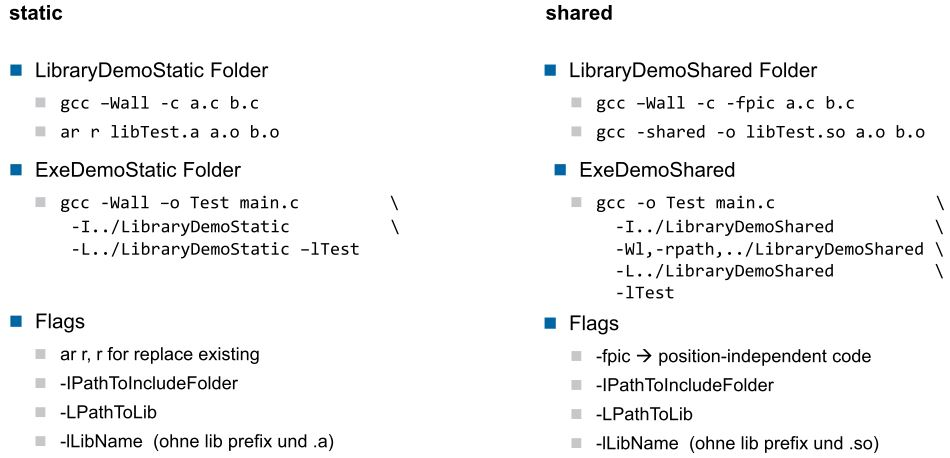
\includegraphics{Figures/createlibrary}}
 
\subsection{Projektstruktur  (siehe Prakti 1)}
\textbf{Für Executable} \\
build: Alle object-Files und executable Files (*.o*) \\
libs: Alle nicht System-Libraries (*.a, *.so, *.h) \\
src: Source Code der Applikationen (*.c, *.cpp, *.h) \\

\textbf{Für Libraries} \\
include: Extern verfügbare Header der Library, API (*.h) \\
lib: Library file der zu buildenden library (*.a, *.so) \\
src: Source code der Library inclusive private Header (*.cpp, *.c, *.h)


